\documentclass[conference]{sig-alternate}
\usepackage{graphicx}
\usepackage{times}
\usepackage{subfigure}
\usepackage{hyperref}

\begin{document}


%\author{\IEEEauthorblockN{Erik Meijer and Georgios Gousios}
%\IEEEauthorblockA{
%Software Engineering Research Group\\
%Delft University of Technology\\
%Delft, The Netherlands\\
%Email: \{h.j.m.meijer, g.gousios\}@tudelft.nl
%}
%}

\title{Teaching Applied Functional Programming\\
\small{Experiences from the functional programming course at TU Delft}
}

\numberofauthors{2}

\author{
\alignauthor
Erik Meijer\\
       \affaddr{Delft University of Technology}\\
       \affaddr{Delft, The Netherlands}\\
       \email{h.j.m.meijer@tudelft.nl}
\alignauthor
Georgios Gousios\\
       \affaddr{Delft University of Technology}\\
       \affaddr{Delft, The Netherlands}\\       
       \email{g.gousios@tudelft.nl}
}

\maketitle

\begin{abstract}

  Recently, the popularity of functional programming as a way of
  solving computational problems has increased significantly. While most
  computer science curricula do include a course on functional programming, in
  many cases it is disconnected from practical applications, which is
  precisely where functional programming shines. To fill in this gap, we
  designed a functional programming course that required students to
  learn by experience in real world applications. In this paper, we present
  the course's design and outline our experience from delivering it.

\end{abstract}

\category{K.3.2}{Computing Milieux}{Computers and Education}[Computer and Information Science Education]
\category{D.1.1}{Software}{Programming Techniques}[Applicative (Functional) Programming]

\terms{Languages}

\keywords{functional programming, teaching}

\section{Introduction}

Due to a variety of reasons, including the advent of cloud computing, the rising
rate of information production and the necessity to reach the market fast,
currently, large corporations and start-ups alike are investigating alternative
programming and information storage models. As a result, during the last few
years, the leading edge of practical software engineering field is witnessing a
slight but noticeable shift towards functional programming ({\sc
fp}).\footnote{See, for example, the reactive manifesto:
\href{http://www.reactivemanifesto.org/}{http://www.reactivemanifesto.org/}}
Scripting languages, notably Javascript and Ruby, pioneered the introduction of
functional concepts, such as closures and lambda functions, to mainstream
programming. A new wave of programming languages, developed to overcome the
expressiveness and complexity limitations exhibited in mainstream languages,
have promoted functional constructs, such as type safe pattern matching, higher
order functions and single assignment variables, to first class citizens (Scala,
{\sc c\#}).  New, functional languages have emerged to fill in the remaining
gaps (F\#, Clojure, Racket), often introducing significant advancements in their
field of specialisation (such as Erlang in distributed fault-tolerant systems).
Finally, large scale information processing systems such as
Map/Reduce~\cite{Dean04} and reactive programming~\cite{Meije12} and domain
specific languages such as {\sc linq}~\cite{Meije11} have integrated functional
concepts to ease the expression of massively parallel computations.

Strictly speaking, {\sc fp} is a style of programming in which the primary
method of computation is the application of functions to arguments.  Among other
features, functional languages offer a compact notation for writing programs,
powerful abstraction methods for structuring them, and a simple mathematical
basis that supports reasoning. Many of the advanced techniques in modern
functional languages, such as monads~\cite{Wadle93} and
catamorphisms~\cite{Meije91}, are closely based on principles from category
theory such as functors, initial algebras, monads and Kleisli categories.

While {\sc fp} has been taught for long in computer science
departments~\cite{Joost93}, curricula tend to emphasize {\sc fp} theory rather than practical applications. Special programming languages are
used to teach {\sc fp} specific concepts, while little connection
is made to how those concepts can be transfered to solving practical software
engineering problems.

The presented course runs at TU Delft for two consecutive years. Our goal, and
the course's moto, is to teach students to  ``think like ({\sc fp})
fundamentalists and code like hackers''. The method we follow is teaching
{\sc fp} principles in the classroom and then expecting students
to apply those concepts in challenging practical projects. The course has a very
strong teaching by example focus: students are expected to participate in both
in-classroom exercises, homework assignments and implement a real world system
as a final project, all within a half-semester (6 -- 8 weeks). 


\section{Challenges}

While planning the course, we dealt with the following challenges related
to the course's organization and content.

\subsection{Heterogeneous background of participants}

The {\sc fp} course is elective at the MSc level. Students from
all departments in the Electrical Engineering, Mathematics and Computer science
faculty are allowed to participate. In the first year, we restricted the
enrollment to the course to 15 participants; we lifted this
restriction during the second year, as we found that the format could allow for
more students to participate.

From the students that enroll, most have received formal introduction to
imperative and object oriented programming in their bachelors curriculum, while
through participation to other courses they had limited exposure to {\sc fp}
(i.e. Map/Reduce in the Web Information Systems course). Some students are
majoring in computer engineering, which meant that their programming experience
was more restricted. Most students also have work experience as programmers as
part of their industrial placement or through participation to start up
ventures.

The diverse backgrounds of the students guarantees that no ge\-ne\-ric
introduction to the topic would be sufficient. For this reason, we decided
to adopt a hands-on-first approach; the students would have to learn by
flexing their programming muscles, instead of being gently introduced to 
the theory through toy examples. During the lectures, we made clear to the
students that it is the delta in learning that we expect them to
demonstrate rather than impressive technical achievements.

\subsection{Choosing the appropriate topics}

{\sc fp} is arguably one of the oldest programming paradigms. In
it is purest form, it is based on a minimalistic theoretical background
($\lambda$-calculus). Relatively recent formulations~\cite{Meije91, Wadle93}
also introduced concepts from category theory. While the every day use of
{\sc fp} does not necessarily require the programmer to be aware
of the theory, understanding it usually leads to more elegant algorithmic
solutions. Teaching {\sc fp} is also associated with advanced type
systems; indeed, the flagship {\sc fp} languages (Haskell, Scala) both offer very sophisticated support for types. Consequently,
teaching the full spectrum of {\sc fp} theory and techniques is impossible in a half-semester course; instead we focus on
practical aspects of data processing, transformations and state representation
using functional techniques.

\subsection{Choosing a programming lan\-guage}

Programming languages, in addition to enabling the programmer to express a
series of instructions to be executed by a computer, affect the programmer's
thought process and consequently her approach towards problem
solving~\cite{Ivers80}.  When teaching a programming course, it is important to
be able to demonstrate concepts without interference by the chosen language's
syntax. However, a non-practical language might have the opposite effect; our
experience has shown that the further a demonstration language is from practical
application, the less important students feel the taught concepts are.
Fortunately, most {\sc fp} concepts can be expressed cleanly by
several widespread languages: for example, Ja\-va\-script, Ruby and {\sc c\#} have
closures, first class and higher order functions, while a number of emerging
languages, such as Scala, Racket, {\sc f\#} and Clojure are functional languages
implemented on familiar development platforms. Apart from staying compatible
with the existing literature, there is no practical reason that necessitates
teaching in a strict {\sc fp} language like Haskell or {\sc ml}.

The above led us to not choose any particular language for the course.  During
the lectures, the demonstration languages where Haskell, {\sc c\#} and {\sc php}, while at the labs we used Scala. We actively encouraged students to use the language of
their choice on the platform of their choice to carry out homework assignments
and the course's final project.

\section{The Course}

The high level goal of the course was to teach the principles of {\sc fp}, and the corresponding Category theoretical principles. More specifically, the educational purposes of the course were:

\begin{itemize}

  \item To introduce students to basic {\sc fp} concepts,
    higher order functions, monads and advanced type systems.

  \item To introduce students to the approach of expressing data processing
    problems as a series of function applications.

  \item To explain the application of functional concepts in non-purely
    functional environments.

\end{itemize}

The course consists of a series of lectures. In total, the
course consisted of 15 hours of lectures. 
The students
also have to carry out a series of optional homework assignments and a final project.
The evaluation is based on student performance on the final assignment. 
The lectures take place in a quarter (half semester), during 6 intense 
weeks; the students have another 2-3 weeks to finish their final projects.

\subsection{Lectures}

The lectures covered the following topics:

\begin{itemize}

  \item Functions and functional composition, higher order functions, recursion, 
    avoiding recursion via higher order functions.

  \item Basic types, function types, currying.

  \item Lists, mapping and traversal using folds.

  \item Monads, composition and their application on the {\sc linq} query 
    language~\cite{Meije11}.

  \item Monoids, functors and their application on data structure processing.

  \item Functional formalization of the Map/Reduce data processing
    paradigm~\cite{Lamme08}.

\end{itemize}

The lecture material was loosely based on Graham Hutton's functional programming
course at the University of Nottingham. The course's recommended book was
Programming in Haskell by the same author~\cite{Hutto07}.

\subsection{Student projects}

At the end of the lecture period, the students were given a selection of
projects to work on. The projects included:

\begin{itemize}

  \item Real time graph visualisation on steaming data.

  \item Haskell constructs (e.g. the Prelude or abstract data types) in Javascript or even {\sc php}. 

  \item Interpreters and byte code converters between languages.

  \item Simple constraint solvers and machine learning algorithms.

  \item Asynchronous request processing in network servers

\end{itemize}

To counterbalance the differences in student experience level, the assignments
are open ended; students can drive their projects as far as they are willing to,
as long as the experience is pleasant enough to allow them to learn. The deliverables for the
assignments are a repository with the source code and short report describing
the solution that the students came up with. The students are also required to
present a working demo by the end of the course time. 

\subsection{Labs}

In the first year it was offered, the course included lab sessions.  The purpose
of the lab sessions were to help students carry out their final assignments and
further explain concepts that might not be clear to them.  Students convened
every week, presented their progress and discussed with each other and with the
lab demonstrator design and practical issues that hindered the implementation of
their projects. To further motivate students to work on their projects, one of
the lab sessions was converted to a full day coding sprint. However, we found
out that participation was diminishing and the sessions were not of much interest to the students,
who preferred to have more time to work on the projects. We therefore canceled
the lab sessions in the course's second year. 

\subsection{Organizing the work}

The higher number of students in the second year of the project made the
organization of student work challenging. To better organize and observe the
student's work, we made active use of Github. Github is a code hosting site that
includes social networking features (such as notifications on events, following
of projects etc) and a dashboard to observe them. We created an organization for
the course\footnote{\href{https://github.com/organizations/fptudelft}{https://github.com/organizations/fptudelft}} and in it we
created repositories for the projects shared among all students registered on
the course. We also created a specialized repository for answering general
questions about the course, using the repository's issue tracking facility.

Github's notification functionality enabled us and the teaching assistants to
answer questions about the student projects in almost real time. We could also
observe work done by the students while it was done and this allowed us to
formulate an early opinion on their progress. We then informally discussed this with the students during idle time (e.g. lecture breaks), giving two types of feedback: praise to students who were doing good, help and support to students that were struggling. 

\section{Experiences}

\subsection{Teaching by example}

The focus of teaching was to present {\sc fp} from a practical
aspect; we were mostly interested to teach students what they can do rather than
the theory behind functional constructs. An important distinction that was made
early on was that the world is imperative; therefore while {\sc fp} 
 can be a great tool for thinking about a problem, a pure functional
solutions cannot reflect on the real world. As a consequence, it is usually best
to mix programming paradigms, i.e. imperative or object-oriented programming for
state representation and {\sc fp} for data processing. In our
experience, this distinction helped students understand that they are already
doing {\sc fp} without noticing; enforcing data immutability to
handle multi-threading problems or passing function arguments in scripting
languages are applications of {\sc fp} principles. The moment
students realized this, their attention was captured to the lectures.

During both lectures and labs, all non-whiteboard examples where actually
entered in a real programming environment (LinqPad in {\sc c\#} or the Scala
command line read-evaluate loop) and the results of the evaluation where
discussed with the students. Participation was encouraged by modifying the
examples and asking the students to perform the evaluation, before the example
was executed.
The examples varied from list manipulation with higher-order
functions to a toy actor model example.
Moreover, we made extensive use of the whiteboard to demonstrate abstract
concepts like type inference and combinators. Typically, we would
write a function signature in Haskell and then expected students to come up 
with its implementation and vice versa.

Of particular interest to the students was the presentation of monads. The
students were teased that they will learn monads in no less than 6 different
ways. Those included presentations of the formal theoretical concepts,
visualizations of monads as blenders (based on the monadic property that once a
value is captured, it is then contained), applications in Haskell for
encapsulating state (through the \textsf{Maybe} monad), applications to generic
programming in {\sc c\#}, applications to {\sc linq} and the reactive extensions
frameworks, and, finally, a whiteboard exercise where students were prompted to
participate in the ad-hoc specification of Haskell's \textsf{IO} monad from
basic principles. Once again, the examples enabled the students to understand
the composition and state containment properties of an otherwise difficult to
comprehend theoretical concept.

\subsection{The teapot exercise}

\begin{figure*}
\centering
\label{fig:teapots}
\subfigure[Input model]{
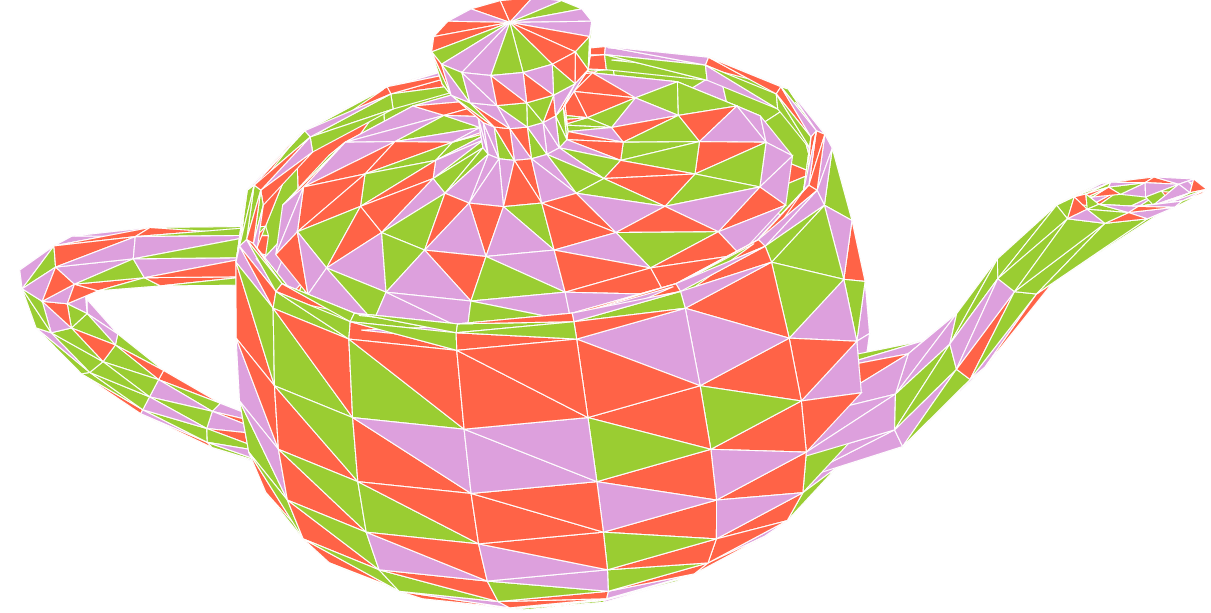
\includegraphics[scale=0.14]{reference.png}
\label{fig:teapot-reference}
}
\subfigure[Decomposed model]{
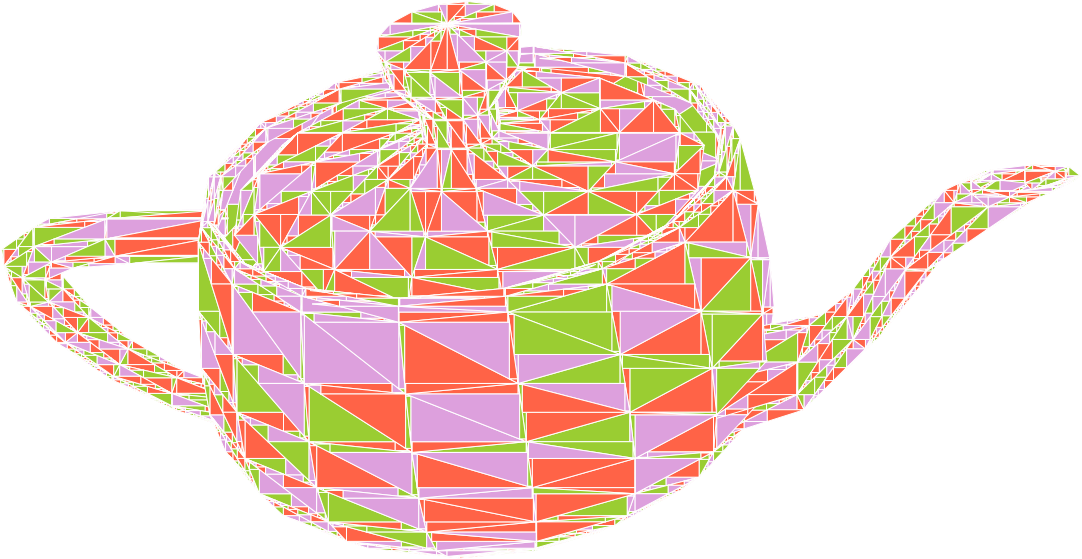
\includegraphics[scale=0.20]{decomposed.png}
\label{fig:teapot-scala}
}
\subfigure[Detail: The teapot's handle]{
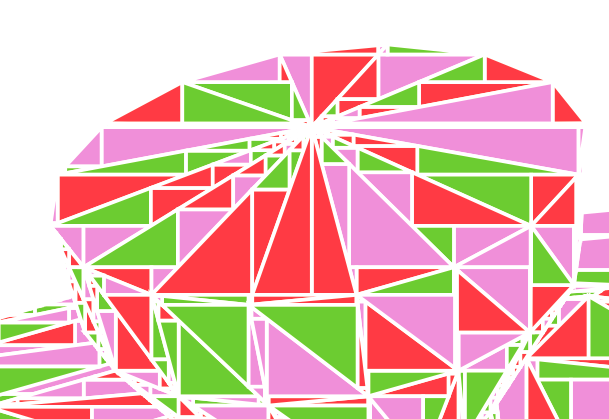
\includegraphics[scale=0.20]{detail.png}
\label{fig:teapot-scala}
}

\caption[]{The teapot input and decomposition results}

\vspace{-1.5em}
\end{figure*}

One of the highlights of the taught period of the course was the teapot
exercise, which we used it to draw the student's attention to the following
facts:

\begin{itemize}

  \item Most modern programming languages can express {\sc fp} constructs.

  \item {\sc fp} works best in data transformation scenarios.

  \item Complex problems can be solved by decomposing them into smaller and simpler ones.

\end{itemize}

The first time the course was given, the exercise consisted of rendering the
Utah Teapot~\cite{Torre06} using any graphics primitive of the student's choice
using only right triangles with one horizontal leg (see
Figure~\ref{fig:teapots}). In its core, the exercise required students to
decompose a collection of arbitrary triangles, which comprised the input Utah
Teapot model, to a collection of right triangles~\cite{Beckm13}. The students
had to come up with the decomposition method (using analytical geometry), a decomposition termination criterion to
stop the decomposition when triangles were too small to be rendered on screen
and a method to recursively apply the above mentioned transformations on the
input data. As always, the students could decide the implementation language of
their choice. The exercise was given as a mid-week homework assignment, between
the Monday and the Friday lectures.

During the second run of the course, the exercise was optimizing decomposition
rather than implementing it. We provided the students with a basic implementation in {\sc php} and asked them to optimize the code by applying new algorithmic techniques and taking into account new language features implemented in a 
pre-release version of Facebook's {\sc php} language version (codenamed Hack).
To further motivate them, we converted the exercise to a programming
contest with prizes for the winning team.

Both times, the students' response was overwhelming. Even though it was made
clear that the exercise would not contribute to the final grade, the will to
apply the data processing techniques taught during the lectures motivated the
students to work very hard. In the first year, the fact that they were
instructed to use their favourite language enabled them to focus on decomposing
the problem in a series of testable calculation steps rather than meddling with
the intricacies of learning a new language. In spite of the advice, students
were eager to test-drive the newly acquired knowledge using a functional
language; apart from {\sc c\#} and Javascript, solutions were also provided in
Scala, Scheme and Haskell. In the second year, the students learned the
value of clean design and breaking code changes to obtain massive
optimizations~\cite{Gousi13}.

\subsection{Map/Reduce}

According to many students, the Map/Reduce data analysis framework was what
drove them to attend the course. In the first year, the lecture on Map/Reduce featured an invited
talk by Prof. Ralf L\"ammel, who presented his formulation of Map/Reduce using
functional programming principles~\cite{Lamme08} and explained how those can be
applied to process semi-structured data. The talk resonated to students; in
their projects, students used implicit, through the selected language's library
collection methods, or explicit, by formalizing data processing as a series of
in memory Map/Reduce operations, forms of Map/Reduce to process their datasets.
Out of personal interest, one student even implemented L\"ammel's Map/Reduce
formulation in Scala, and through the language's extension mechanisms, adapted
it for use as an extension method by any Scala collection type, including
parallel collections. 

\subsection{The coding sprint day}

Coding sprints or ``hackathons'' have long been used by open source software
projects to speed up development and increase participation of community
members. In a typical sprint, project members set measurable
targets and work intensively in a tight deadline to deliver them. To ensure the
timely delivery of the student projects, we organized an one day coding sprint,
during which the students were requested to i) set explicit targets ii) write
code for 7 hours with a short break iii) present a 5 minute demo of their work
at the end of the day. All project teams where expected to work in the same
room, while communication among the teams was facilitated by the lab
demonstrator, to avoid unnecessary distractions.

Interestingly, the coding sprint was organized on student request. The reason
was that pressure from other courses did not allow them to be together as teams.
The sprint taught students the importance of setting realistic development goals
and the necessity of iterative development. Even though all teams were off
target at the end of the day, most were able to create a rough prototype in less
than 7 hours, using functional programming techniques. 

%\subsection{The student projects}
%
%For implementing their projects, the students selected languages and frameworks
%that are currently emerging and popular among non-traditional software
%development environments. All students did their projects in either Scala or
%Javascript, with one exception, using frameworks such as Akka (for actors),
%Scalatra (for implementing {\sc rest} {\sc api}s) or Node.js (for server-side
%processing). From the implementations it appears that students did apply
%their 
%
\section{Conclusion}

Teaching the concepts of solving problems algorithmically can be a daunting
task~\cite{Futsc06}; especially more so, when the subjects are already in a
specific mindset. The assumption of the presented course was that imperative and
functional programming are really the two sides of the same coin; by focusing on
how students can apply rather than just be taught concepts of functional
programming using the, typically imperative, languages they already know, allows
them to better appreciate the strong points and weaknesses of each paradigm. In
our experience, the approach has been successful. Both throughout the initial
homework assignments and in their projects, the students demonstrated a high
degree of appreciation of functional programming concepts. Above all, we
believe that it was the hands-on approach 
employed in this course that allowed students to sharpen their skills and
understand the concepts that were taught during it.

\section*{Acknowledgements and Availability}
We would like to thank the course participants for their enthusiasm and
dedication. The source code to all student projects and the teapot
exercise can be found at (or linked from) \href{https://github.com/organizations/fptudelft}{https://\-github.com\-/organizations\-/fptudelft}. This work is partially supported by Marie Curie {\sc ief} 298930 -- {\sc sefunc}.

\bibliography{paper}
\bibliographystyle{abbrv}
\end{document}

